Solutions courtesy of Richard Li.

\subsection*{Problem 16}
\begin{proof}
We first hope to prove that in every 2-coloring of the edges of the complete bipartite graph $K_{5,5}$ there is a monochromatic $K_{2,2}$.
Suppose our graph is $A \sqcup B = K_{5,5}$ with colors red and blue.
Consider some $v_1 \in A$, and look at the 5 edges leaving $A$. Some color makes up at least three of these edges. Without loss of generality assume it is red. We now have two cases. Either there exists some $v'$ such that two of the vertices connected to $v_1$ with red edges are also connected to $v'$, in which case there is a red $K_{2,2}$, or there is no such vertex. If there is no such vertex $v_2$, this means that for each $v_i \in A$, $i \neq 1$, there are at least two blue edges from the at least three vertices connected to $v_1$ with a red edge. However, see that since $\binom{3}{2} = 3$, at least one choice of two edges must be repeated among two different vertices, $v_i$ and $v_j$, which is a blue $K_{2,2}$ as desired. The same statement is not true for $K_{5,4}$. Consider the following graph:
\begin{center}
    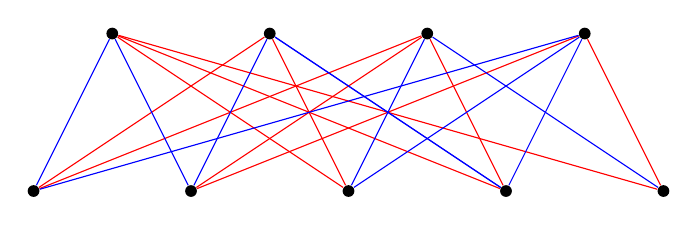
\begin{tikzpicture}[scale=2, every node/.style={circle, fill, inner sep=1.5pt, draw=none}]
        % Top row (4 vertices)
        \node (t1) at (-3/2, 1) {};
        \node (t2) at (-1/2, 1) {};
        \node (t3) at (1/2, 1) {};
        \node (t4) at (3/2, 1) {};

        % Bottom row (5 vertices)
        \node (b1) at (-2, 0) {};
        \node (b2) at (-1, 0) {};
        \node (b3) at (0, 0) {};
        \node (b4) at (1, 0) {};
        \node (b5) at (2, 0) {};

        \draw[red] (t1) -- (b3);
        \draw[red] (t1) -- (b4);
        \draw[red] (t1) -- (b5);

        \draw[red] (t2) -- (b1);
        \draw[red] (t2) -- (b3);

        \draw[red] (t3) -- (b1);
        \draw[red] (t3) -- (b2);
        \draw[red] (t3) -- (b4);

        \draw[red] (t4) -- (b2);
        \draw[red] (t4) -- (b5);

        
        \draw[blue] (t1) -- (b1);
        \draw[blue] (t1) -- (b2);

        \draw[blue] (t2) -- (b2);
        \draw[blue] (t2) -- (b4);
        \draw[blue] (t2) -- (b4);

        \draw[blue] (t3) -- (b3);
        \draw[blue] (t3) -- (b5);

        \draw[blue] (t4) -- (b1);
        \draw[blue] (t4) -- (b3);
        \draw[blue] (t4) -- (b4);
    \end{tikzpicture}
\end{center}

\end{proof}

\subsection*{Problem 17}

\begin{proof}
We hope to show that $R(p,q) \leq \binom{p+q-2}{p-1}$.
To do so, we use strong induction on $p + q$. For our base case, note that for $p = 1$, $R(1,q) = 1$, and $\binom{1 + q-2}{0} = 1$. The same holds for $q = 1$. So, suppose the inequality holds for all $p',q'$ such that $p' + q' < p + q$.
See that $R(p,q) \leq R(p-1,q) + R(p,q-1)$
where, by our inductive hypothesis
$R(p,q) \leq \binom{p+q-3}{p-2} + \binom{p+q-3}{p-1}.$
Then, since
$\binom{p+q-3}{p-2} + \binom{p+q-3}{p-1} = \binom{p+q-2}{p-1}$
we have that
$R(p,q) \leq \binom{p+q-2}{p-1}$
as desired.
\end{proof}

\subsection*{Problem 18}

\begin{proof}
We hope to prove that $R_3(4,4) \leq 19$.
To do so, we use the identity that
$R_{t+1}(p,q) \leq R_t(R_{t+1}(p-1,q), R_{t+1}(p,q-1))+1.$
So, we have that
$R_{3}(4,4) \leq R_2(R_{3}(3,4), R_{3}(4,3))+1.$
Notably, $R_3(3,4) = R_3(4,3) = 4$ since $K^3_3$ can simply have a red edge, but $K^3_4$ must either be monochromatic red, or contain a blue edge which is a monochromatic blue $K_3^3$.
So,
$R_{3}(4,4) \leq R_2(4, 4)+1 = 18 + 1 = 19$
as desired.
\end{proof}

\subsection*{Problem 19}

\begin{proof}
We hope to prove that $R(n) \leq R_3(6,n)$.
To do so, consider the graph $K_{R_3(6,n)}$ and any edge coloring on it, say $C$.
We now construct an edge coloring of $K_{R_3(6,n)}^3$ as follows. We color an edge blue if the corresponding vertices in $C$ form a monochromatic triangle. Otherwise, we color the edge red. See that it is impossible to have a red $K_6$, since this would imply that within 6 vertices, there exists no monochromatic $K_3$ in $C$, which is impossible since $R(3) = 6$.
So, there exists some blue $K^3_n$. See that this must correspond to a monochromatic $K_n$ in our coloring $C$ since if there were two different colors, there would be some red edge.

\end{proof}

\subsection*{Problem 20}

\begin{proof}
We hope to prove that a simple intersecting hypergraph on $n$ vertices has at most $2^{n-1}$ edges.
To see why this is the case, see that we have $2^n$ possible edges, since this is the cardinality of the power set of $[n]$ elements. Then, see if we have some $e \in E$, $e^C \notin E$ since $e \cap e^C = \varnothing$.
Hence, since every element has a unique complement, we can have at most half the $2^n$ possible edges, which is $2^{n-1}$.

\end{proof}